% Options for packages loaded elsewhere
\PassOptionsToPackage{unicode}{hyperref}
\PassOptionsToPackage{hyphens}{url}
\PassOptionsToPackage{dvipsnames,svgnames*,x11names*}{xcolor}
%
\documentclass[
  12pt,
]{article}
\usepackage[]{mathpazo}
\usepackage{setspace}
\usepackage{amssymb,amsmath}
\usepackage{ifxetex,ifluatex}
\ifnum 0\ifxetex 1\fi\ifluatex 1\fi=0 % if pdftex
  \usepackage[T1]{fontenc}
  \usepackage[utf8]{inputenc}
  \usepackage{textcomp} % provide euro and other symbols
\else % if luatex or xetex
  \usepackage{unicode-math}
  \defaultfontfeatures{Scale=MatchLowercase}
  \defaultfontfeatures[\rmfamily]{Ligatures=TeX,Scale=1}
\fi
% Use upquote if available, for straight quotes in verbatim environments
\IfFileExists{upquote.sty}{\usepackage{upquote}}{}
\IfFileExists{microtype.sty}{% use microtype if available
  \usepackage[]{microtype}
  \UseMicrotypeSet[protrusion]{basicmath} % disable protrusion for tt fonts
}{}
\makeatletter
\@ifundefined{KOMAClassName}{% if non-KOMA class
  \IfFileExists{parskip.sty}{%
    \usepackage{parskip}
  }{% else
    \setlength{\parindent}{0pt}
    \setlength{\parskip}{6pt plus 2pt minus 1pt}}
}{% if KOMA class
  \KOMAoptions{parskip=half}}
\makeatother
\usepackage{xcolor}
\IfFileExists{xurl.sty}{\usepackage{xurl}}{} % add URL line breaks if available
\IfFileExists{bookmark.sty}{\usepackage{bookmark}}{\usepackage{hyperref}}
\hypersetup{
  colorlinks=true,
  linkcolor=blue,
  filecolor=Maroon,
  citecolor=Blue,
  urlcolor=Blue,
  pdfcreator={LaTeX via pandoc}}
\urlstyle{same} % disable monospaced font for URLs
\usepackage[margin=1in]{geometry}
\usepackage{graphicx}
\makeatletter
\def\maxwidth{\ifdim\Gin@nat@width>\linewidth\linewidth\else\Gin@nat@width\fi}
\def\maxheight{\ifdim\Gin@nat@height>\textheight\textheight\else\Gin@nat@height\fi}
\makeatother
% Scale images if necessary, so that they will not overflow the page
% margins by default, and it is still possible to overwrite the defaults
% using explicit options in \includegraphics[width, height, ...]{}
\setkeys{Gin}{width=\maxwidth,height=\maxheight,keepaspectratio}
% Set default figure placement to htbp
\makeatletter
\def\fps@figure{htbp}
\makeatother
\setlength{\emergencystretch}{3em} % prevent overfull lines
\providecommand{\tightlist}{%
  \setlength{\itemsep}{0pt}\setlength{\parskip}{0pt}}
\setcounter{secnumdepth}{-\maxdimen} % remove section numbering
\usepackage{hyperref}
\usepackage[]{natbib}
\bibliographystyle{plainnat}

\author{}
\date{\vspace{-2.5em}}

\begin{document}

\setstretch{1}
\begin{flushright} 
    \end{flushright}
    \begin{center} \textbf{Parlr: Parallelized Record Linkage in R} \linebreak
    \textbf{Technical Appendix}
    
    Brian Kundinger
    
    April 23, 2021
    
    STA 561

    \end{center}

\hypertarget{notation-and-assumptions}{%
\subsection{Notation and Assumptions}\label{notation-and-assumptions}}

Denote two files as \(A\) and \(B\), with \(n_A\) and \(n_B\) records
respectively, with records indexed as \(i \in \{1, \ldots, n_A\}\) in
\(A\) and \(j \in \{1, \ldots, n_B\}\) in \(B\). Without loss of
generality, label the files such that \(n_A \geq n_B\). We also assume
there are no duplicates within files, only across.

For each record pair under consideration, we generate a comparison
vector
\(\boldsymbol{\gamma}_{ij} = \{\gamma_{ij}^1, \ldots, \gamma_{ij}^F\}\),
where \(F\) is the number of fields used in the linkage and each
\(\gamma_{ij}^f\) takes on a value \(l \in \{1, \ldots, L_f\}\)
indicating the level agreement between the two records on a specified
field. For ease of modeling and computation, we restrict these
similarity scores to be discrete, ordinal variables, and the
construction of these is left to the modeler. With notation
\(\gamma_{ij}^f \in \{0, \ldots, L_f - 1\}\) for the number of possible
agreement levels for field \(f\), we use binary 0-1 variables to
indicate exact matching, and 0-1-2 variables to provide an option for
partial matching. For text data, we calculate similarity based on
Levenstein distance or some other text similarity score, and bin these
scores to integers for use in the model.

To indicate matching status, we adopt the \emph{linkage structure
parameter} \(\mathbf{Z} = (Z_1, \ldots, Z_{n_B})\) from Sadinle 2017,
defined as \[Z_j=\begin{cases} 
    i,  & \text{if records } i\in A \text{ and } j\in B \text{ refer to the same entity}; \\
    n_A + 1,  & \text{if record } j\in B \text{ does not have a match in file } A; \\
\end{cases}\] This provides more memory efficient storage for the
linkage information than a \(n_A \times n_B\) sparse matrix of
indicators.

Following the Fellegi Sunter framework, we define
\(m^{fl}:= P(\gamma_{ij}^f = l |Z_j = i)\) to be the probability of
observing agreement level \(l\) in field \(f\) for records \(i\) and
\(j\) given that the records are a match, and similarly define
\(u^{fl}:= P(\gamma_{ij}^f = l |Z_j \neq i)\), for non-matches. We also
adopt Fellegi and Sunter's conditionally independent fields assumption
that the level of agreement on one field is independent of the level of
agreement on another. Though this assumption is often not reasonable
(for example, first name and gender are two clearly dependent fields),
but it is common within the record linkage literature and generally
leads to models that perform well in practice; see discussion for
further remarks. Lastly, we define \(\lambda\) to be the (marginal)
probability that some record \(j \in B\) has a match in \(A\).

Wherever possible, we reserve superscripts for denoting field and level,
while reserving subscripts for record indices. For example,
\(\mathbf{m}^f = (m^{f1}, \ldots, m^{fL_f})\) is the probability
distribution governing field \(f\) for matching records, and
\(\mathbf{m}_{ij}= \prod_{f=1}^{F}\prod_{l=1}^{L_f} \left(m^{fl}\right)^{\mathbf{1}_{\gamma_{ij}^f = l}} = P(\boldsymbol{\gamma}_{ij}|Z_j = i)\)
is the product of the appropriate \(\mathbf{m}\) parameters for record
pair \((i,j)\). We hope that these conventions avoid overloaded notation
in the likelihood and subsequent derivations.

\hypertarget{model-specification}{%
\section{Model Specification}\label{model-specification}}

For fields \(f \in \{1, \ldots, F\}\) and levels
\(l\in \{1, \ldots, L_f\}\) we adopt the following likelihood and prior
distributions.

\[P(\Gamma|\mathbf{Z}, \mathbf{m}, \mathbf{u}, \lambda) =\prod_{j=1}^{n_B}  \prod_{i=1}^{n_A}\mathbf{m}_{ij}^{\mathbf{1}_{z_j = i}}\mathbf{u}_{ij}^{\mathbf{1}_{z_j \neq i}}\]

\[\mathbf{m^{f}} \sim \text{Dirichlet}(\alpha^{f1}, \ldots, \alpha^{fL_f})\]
\[\mathbf{u^{f}} \sim \text{Dirichlet}(\beta^{f1}, \ldots, \beta^{fL_f})\]
\[Z_j | \lambda =
\begin{cases} 
    \frac{1}{n_A}\lambda  & z_j \leq n_A; \\
     1-\lambda &  z_j  = n_A + 1 \\
\end{cases}\]

\[\lambda \sim \text{Beta}(\alpha_{\lambda}, \beta_{\lambda}) \] The
prior for \(Z_j\) has equal probability of matching to all records
\(i\in A\), and non-matching probability governed by \(\lambda\).
Therefore a \(\lambda \sim \text{Beta}(1, 1)\) corresponds to a prior
belief that nonmatches and matches are equally likely, and a
\(\lambda \sim \text{Beta}(1, \frac{1}{n_A})\) prior corresponds to a
uniform prior on the labeling of \(\mathbf{Z}\).

\hypertarget{posterior-sampling}{%
\subsection{Posterior Sampling}\label{posterior-sampling}}

We work with the following factorization of the joint distribution:

\[p(\Gamma, \mathbf{Z}, \mathbf{m}, \mathbf{u}, \lambda) = p(\Gamma|\mathbf{Z}, \mathbf{m}, \mathbf{u}) p(\mathbf{Z} | \lambda) p(\mathbf{m}, \mathbf{u}) p(\lambda)\]

This factorization leads to following Gibbs Sampler:

\underline{Sample $\mathbf{m}^{(s+1)}$ $\mathbf{u}^{(s+1)}|\Gamma, \mathbf{Z}^{(s)}$:}
The \(\mathbf{m}\) and \(\mathbf{u}\) parameters are updated through
standard multinomial-dirichlet mechanics. Thus we have

\[\mathbf{m}^f|\mathbf{Z}, \Gamma \sim \text{Dirichlet}(\alpha^{f1}(\mathbf{Z}), \ldots, \alpha^{fL_f}(\mathbf{Z}))\]
\[\mathbf{u}^f|\mathbf{Z}, \Gamma \sim \text{Dirichlet}(\beta^{f1}(\mathbf{Z}), \ldots, \beta^{fL_f}(\mathbf{Z}))\]
where
\(\alpha_{fl}(\mathbf{Z})= \sum_{i,j} \mathbf{1}_{obs(\gamma_{ij}^f)}\mathbf{1}_{\gamma_{ij}^f = l} \mathbf{1}_{z_j = i}\)
and
\(\beta_{fl}(\mathbf{Z})= \mathbf{1}_{obs(\gamma_{ij}^f)}\mathbf{1}_{\gamma_{ij}^f = l} \mathbf{1}_{z_j \neq i}\).

\underline{Sample $\lambda^{(s+1)}|\mathbf{Z}^{(s)}$:} As a function of
\(\lambda\), the linkage structure parameter \(\mathbf{Z}\) is sequence
of successes (when \(z_j < n_A + 1\)) and failures (when
\(z_j = n_A + 1\)), and therefore
\(p(\mathbf{Z}|\lambda) = \mathcal{L}(\lambda|\mathbf{Z})\) is
determined only by the number of duplicates
\(D = \sum_{i=1}^{n_B}\mathbf{1}_{z_j < n_A + 1}\) encoded by
\(\mathbf{Z}\). Thus we have

\[p(\lambda | \mathbf{Z}) \propto p(\mathbf{Z}|\lambda)p(\lambda)\]
\[\propto \lambda^D (1-\lambda)^{n_B - D} \lambda^{\alpha_{\lambda} -1} (1-\lambda)^{\beta_{\lambda} -1}\]
\[ \propto \lambda^{D + \alpha_{\lambda} - 1} (1-\lambda)^{n_B - D + \beta_{\lambda} -1}\]
\[\implies \lambda^{(s+1)}|\mathbf{Z}^{(s+1)} \sim \text{Beta}(D + \alpha_{\lambda}, n_B - D + \beta_{\lambda})\]

\underline{Sample $\mathbf{Z}^{(s+1)}|\Gamma, \mathbf{m}^{(s+1)}, \mathbf{u}^{(s+1)}, \lambda^{(s+1)}$:}
Because we sample \(Z_j\) independently of all other \(Z_{j'}\), we use
only the full conditional for an individual \(Z_j\). Let \(\Gamma_{.j}\)
denote the set of \(n_A\) comparison vectors with \(j \in B\), and note
that as a function of \(Z_j\), the likelihood
\(p(\Gamma_{.j}|Z_j, \mathbf{m}, \mathbf{u}) = \mathcal{L}(Z_j|\Gamma_{.j}, \mathbf{m}, \mathbf{u})\)
is a discrete distribution with probabilities proportional to

\begin{align*}
p(\Gamma_{.j}|Z_j = z_j, \mathbf{m}, \mathbf{u}) &\propto \prod_{i=1}^{n_A}\mathbf{m}_{ij}^{\mathbf{1}_{z_j = i}}\mathbf{u}_{ij}^{\mathbf{1}_{z_j \neq i}}\\
&\propto \prod_{i=1}^{n_A}\left(\frac{\mathbf{m}_{ij}}{\mathbf{u}_{ij}}\right)^{\mathbf{1}_{z_j = i}} && \text{By dividing through by} \prod_{i = 1}^{n_A}\mathbf{u}_{ij}\\
&=
\begin{cases} 
    w_{ij}  & z_j \leq n_A; \\
    1 &  z_j  = n_A + 1 \\
\end{cases}\\
\end{align*}

where
\(w_{ij} = \frac{\mathbf{m}_{ij}}{\mathbf{u}_{ij}} = \frac{P(\boldsymbol{\gamma_{ij}}|Z_j = i)}{P(\boldsymbol{\gamma_{ij}} |Z_j \neq i)}\).
The interested reader should note that these are precisely the
likelihood ratios used in the Fellegi-Sunter model to classify matches
and non-matches, and we therefore refer to \(w_{ij}\) as the
\emph{Fellegi Sunter weights}.

With the likelihood in this form, we can derive the full conditional
\[p(Z_j|\Gamma_{.j}, \mathbf{m} ,\mathbf{u}, \lambda) \propto p(\Gamma_{.j}| Z_j, \mathbf{m} ,\mathbf{u}) P(Z_j|\lambda)\]

\[\propto \left(\sum_{i=1}^{n_A}w_{ij}\mathbf{1}_{z_j = i} + \mathbf{1}_{z_j = n_A + 1}\right)\left(\lambda\sum_{i=1}^{n_A}\frac{1}{n_A}\mathbf{1}_{z_j = i} + (1-\lambda)\mathbf{1}_{z_j = n_A + 1}\right)\]
\[= \frac{\lambda}{n_A}\sum_{i=1}^{n_A}w_{ij}\mathbf{1}_{z_j = i} + (1-\lambda)\mathbf{1}_{z_j = n_A + 1} \]
\[ \implies Z_j^{(s+1)} | \mathbf{m}, \mathbf{u}, \Gamma, \lambda \propto
\begin{cases} 
    \frac{\lambda}{n_A}w_{ij}   & z_j \leq n_A; \\
     1-\lambda &  z_j  = n_A + 1 \\
\end{cases}\]

In order to make fair comparisons against the Sadinle 2017 model, we
integrate over the posterior of \(\lambda\) and rearrange terms to
produce the final full conditional:

\[p\left(Z_j^{(s+1)}  = i| \mathbf{m}, \mathbf{u}, \mathbf{Z^{(s)}}\right) \propto
\begin{cases} 
    w_{ij}  & i \leq n_A; \\
     n_A \frac{n_B - D + \beta_{\lambda}}{D + \alpha_{\lambda}} & i  = n_A + 1 \\
\end{cases}\]

\hypertarget{bayes-estimate}{%
\subsection{Bayes Estimate}\label{bayes-estimate}}

Our Gibbs sampler provides posterior samples of \(\mathbf{Z}\) which we
use to make our final decisions about the linkage structure. In the case
where we false matches and missed matches contribute the same loss, we
declare \((i,j)\) to be a match whenever \(P(Z_j = i) > \frac{1}{2}\)
according to these posterior samples. We can create more elaborate
decisions by attributing different loss values to different kinds of
error, and allowing pairings with middling posterior probabilities to be
left unlabeled by the algorithm so that the modeler can address those
manually. For further discussion, see Sadinle 2017.

Since our Gibbs procedure does not strictly enforce one-to-one matching,
it is possible for the final Bayes estimate to link multiple records in
\(B\) to one record in \(A\). The modeler can either report both such
matches (with their respective posterior match probabilities), or
resolve these conflicts by accepting only the match with highest
posterior probability. Rigorous proof of this resolution procedure is
deferred to future work.

\hypertarget{efficient-computation}{%
\section{Efficient Computation}\label{efficient-computation}}

Broadly speaking, we increase our computational efficiency by
recognizing that record pairs contribute to posterior calculations only
through the agreement pattern of the \(\gamma_{ij}\) vector. Let
\(\mathcal{H}\) be the set of unique agreement patterns in the data, let
\(P\) denote the total number of unique agreement patterns. Note that
\(P\) is bounded above by \(\prod_{f=1}^F L_f\), and that this bound
does not scale with \(n_A\) or \(n_B\). We index these agreement
patterns by \(p \in \{1, \ldots, P\}\), and say \((i,j) \in h_p\) when
the \((i,j)\) pair exhibits the \(p^{th}\) agreement pattern. Wherever
possible, we conduct calculations over these \(P\) agreement patterns
rather than the \(n_A \times n_B\) record pairs.

\hypertarget{data-representation-and-hashing}{%
\subsection{Data Representation and
Hashing}\label{data-representation-and-hashing}}

In the classic Fellegi Sunter framework, \(\Gamma\) is a
\(n_A n_B \times F\) matrix, with each row providing the comparison
vector for a different \((i,j)\) pair. We however do not store these
comparison vectors themselves, but instead only the a hashed value
corresponding to the agreement pattern of the \((i, j)\) pair. Enamorado
et al (2019) provided the hashing function
\[\sum_{f=1}^F \mathbf{1}_{\gamma_{(i,j)}^f >0}2^{\gamma_{(i,j)}^f + \mathbf{1}_{f>1} \times \sum_{e=1}^{f-1}(L_e-1)}\]
to map each agreement pattern to a unique value, but packages like
\texttt{dplyr} in \texttt{R} are capable of this as well.

We store this information in a nested list \(\tilde{\Gamma}\) where the
\(p^{th}\) component of the \(j^{th}\) list contains a vector of records
in \(A\) that share agreement pattern \(p\) with record \(j \in B\). For
each \(p\), we also calculate
\(H_p = \sum_{i=1}^{n_A}\sum_{j=1}^{n_B} \mathbf{1}_{(i,j) \in h_p}\),
the total instances of agreement pattern \(p\) throughout the data, and
also for each \(j\), we calculate
\(H_{p_j} = \sum_{i=1}^{n_A} \mathbf{1}_{{(i,j) \in h_p}}\) the
instances of agreement pattern \(p\) among the comparison vectors
between record \(j \in B\) and each of the \(n_A\) records in \(A\).

For large data, we can partition the two datasets \(A\) and \(B\) into
smaller blocks \(\{A_m\}\) and \(\{B_m\}\) for more manageable
computations. On a single machine, we can read-in data sequentially,
conduct hashing, collect results, and delete the original data from
memory before continuing with the next chunk of data. With multiple
cores or multiple machines, this can be done in parallel. Storing this
hashed information still becomes burdensome for large data, but this
hashing method greatly expands the capabilities of the Fellegi-Sunter
framework.

Lastly, the classic Fellegi Sunter method represents the \(\gamma_{ij}\)
comparison vector as vector of length \(F\), with each component
\(\gamma_{ij}^f\) taking on values in \(\{0, \ldots, L_f - 1\}\). To
ease computations, we instead represent the comparison as a
concatenation of \(F\) many binary indicator vectors of lengths \(L_f\).
For example, if \(L_1 = L_2 = 2\) and \(L_3 = 3\), then
\(\gamma_{ij} = (1, 0, 2)\) under the classical framework becomes
\(\gamma_{ij} = (0, 1, 1, 0, 0, 0, 1)\) under our framework. This is a
bijective transformation that does not change the meaning of the data,
but this representation will ease calculations and posterior updates.

\hypertarget{gibbs-sampling}{%
\subsection{Gibbs Sampling}\label{gibbs-sampling}}

After receiving matching statuses from \(\mathbf{Z}\), the Sadinle
method calculates \(\alpha_{fl}(\mathbf{Z})\) and
\(\beta_{fl}(\mathbf{Z})\) for each field and level. This constitutes
\(2 \times \sum L_f\) many summations over \(n_A \times n_B\)
quantities, and becomes computationally burdensome with large data. In
contrast, we recognize that each unique agreement pattern contributes to
the posterior \(\alpha(\mathbf{Z})\) and \(\beta(\mathbf{Z})\) vectors
in the same way. In fact, if we denote
\(H_p^m = \sum_{j=1}^{n_B} \mathbf{1}_{(Z_j, j) \in h_p}\) to be the
number of matching record pairs with agreement pattern \(p\), then the
contribution of pairs of pattern \(p\) to the \(\alpha(\mathbf{Z})\)
vector is simply \(H_p^m \times h_p\). Thus our posterior update for
\(\alpha\) is simply
\(\alpha(\mathbf{Z}) = \alpha_0 + \sum_{p=1}^P H_p^m \times h_p\). Then,
we can easily calculate \(H_p^u\), the number of nonmatching record
pairs of agreement pattern \(p\), by subtracting the number of matching
pairs from the total present in the data; that is
\(H_p^u = H_p - H_p^m\). From this, we can update our \(\beta\)
parameter through
\(\beta(\mathbf{Z}) = \beta_0 + \sum_{p=1}^P H_p^u \times h_p\). Note
that these constitute \(P\) many summations over \(n_B\) quantities, and
thus avoid the \(n_A \times n_B\) summation from the original method.

Sadinle uses a prior for \(\mathbf{Z}\) that induces the a full
conditional for \(Z_j\) that strictly enforces one-to-one matching. In
particular, this sampler removes previously matches records from the set
of candidate records when sampling \(Z_j\), creating a dependency that
makes the sampler \emph{inherently serial}. By weakening the one-to-one
requirement, our full conditional for \(Z\) does not depend on the rest
of the \(\mathbf{Z}_{-j}\) vector, and thus can be computed in parallel.
More importantly, since only the agreement pattern of \(Z_j\) is used
for calculations within the Gibbs sampler, and not the particular record
label, we can conduct this sampling only at the level of the unique
agreement patterns. This boosts computation time far greater than
parallelization.

To do this, we calculate the Fellegi Sunter weight \(w_{h_p}\) for each
unique pattern, sample the agreement pattern between \(j\) and its
potential match, and then sample the record label uniformly among viable
records. More concretely, define \(h(Z_j)\) to be the agreement pattern
between \(j\) and its potential match, and say \(h(Z_j) = h_{P+1}\) when
\(Z_j = n_A + 1\). Then,

\[h\left(Z_j^{(s+1)}\right) | \mathbf{m}, \mathbf{u}, \mathbf{Z^{(s)}} \propto
\begin{cases} 
    w_{h_p}\times H_{p_j}  & p \leq P; \\
     n_A \frac{n_B - D + \beta_{\lambda}}{D + \alpha_{\lambda}} &   p = P + 1 \\
\end{cases}\]

We complete the entire Gibbs procedure at the level of the \(P\)
agreement patterns. After, we can back-fill the records corresponding to
the agreement patterns by sampling uniformly at random among candidate
records stored in \(\tilde{\Gamma}\).

\hypertarget{simulation-studies}{%
\section{Simulation Studies}\label{simulation-studies}}

In his 2017 paper, Sadinle demonstrated the strength of his method by
running \texttt{BRL} on simulated pairs of files with differing levels
of errors and overlap. Comparing our method against \texttt{BRL} on
these same simulated datasets, we find that our method only has weakened
performance in the extreme scenario of very high errors and very high
overlap across files. We use the following measures of accuracy in our
analysis: although using only recall and precision is common in the
literature, we find it useful to have a single metric the gauge overall
performance, and thus also include F measure.

\[\text{Recall} = \frac{\text{Matches Correctly Identified}}{\text{True Matches in Data}}\]
\[\text{Precision} = \frac{\text{Declared Matches}}{\text{True Matches in Data}}\]
\[\text{F-Measure} = 2\left(\frac{\text{Recall} \times \text{Precision}}{\text{Recall} + \text{Precision}}\right)\]

\begin{center}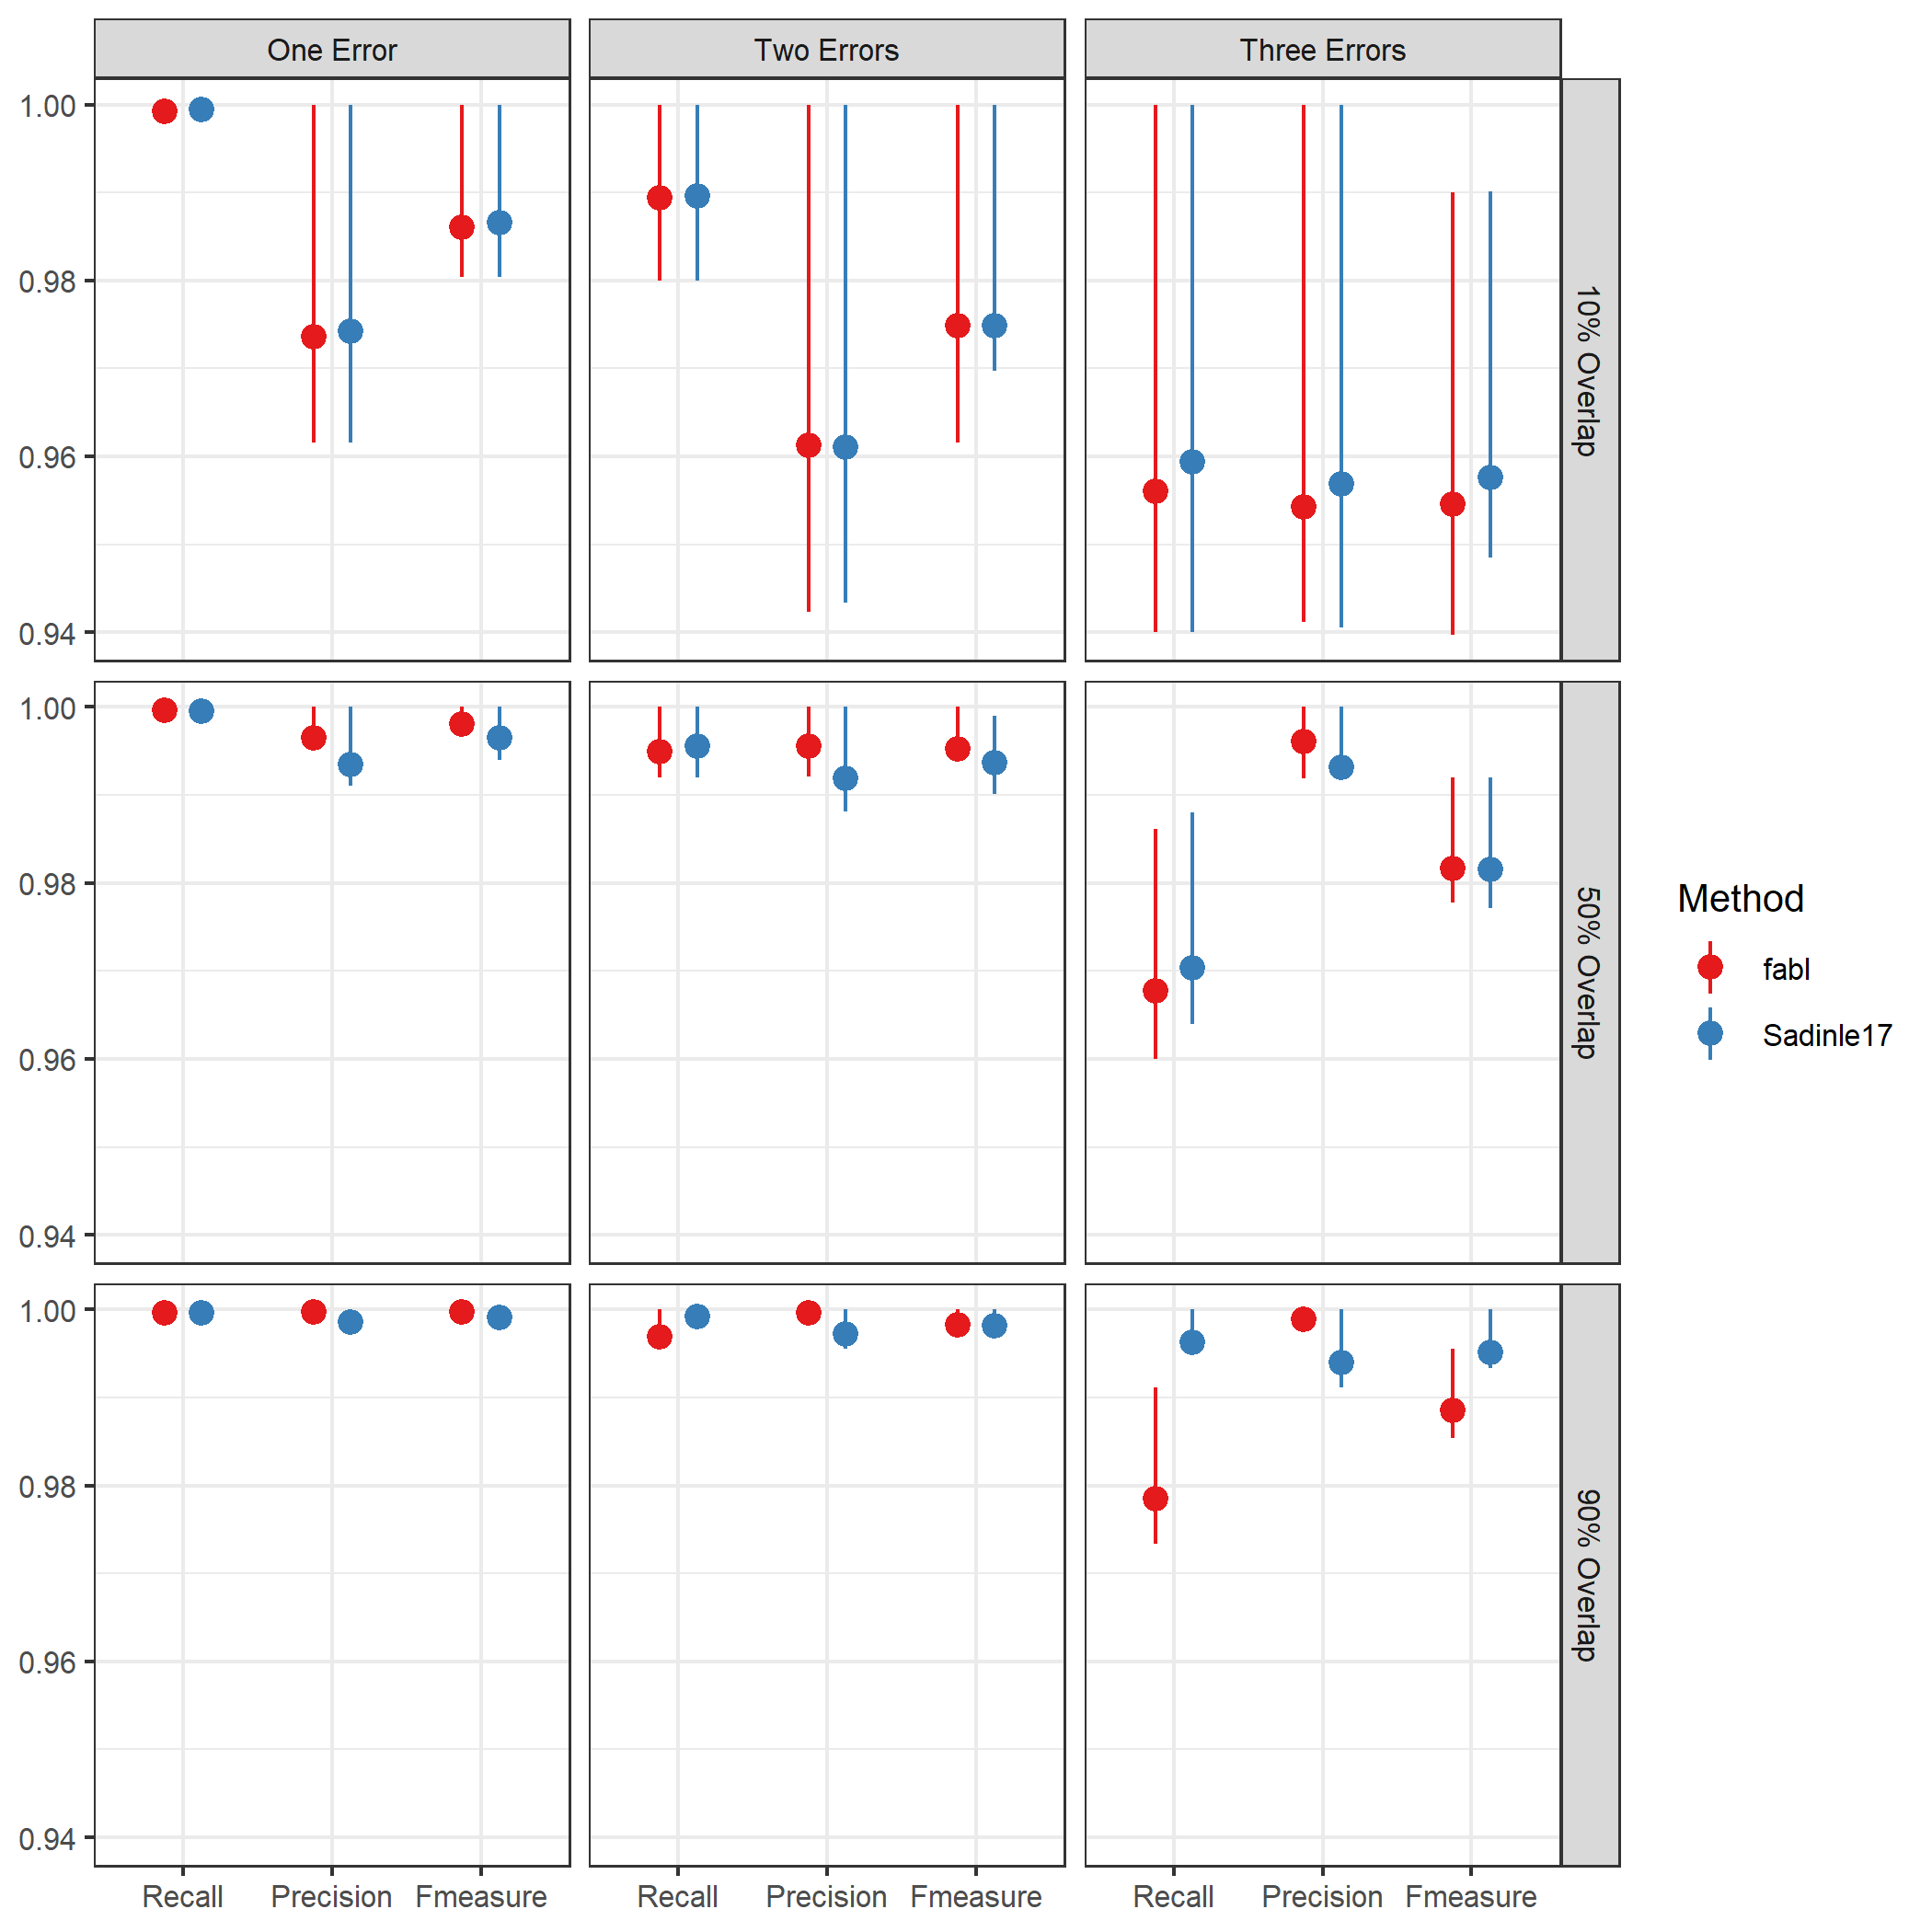
\includegraphics[width=29.17in]{../notes/figures/sadinle_sim_plot} \end{center}

To demonstrate speed, we generate comparison vectors from pre-specified
distributions so that we can easily increase the size of the linkage
problem. Distributions are meant to emulate the behavior of similarity
scores across first name, last name, and day, month, and and year of
birth, with 1 indicating an exact match on a particular field and 0
indicating a nonmatch. We simulate these data for different values of
\(n_A\) and \(n_B\), and compare the runtime of \texttt{parlr} against
\texttt{BRL}. We see that at low data size, \texttt{BRL} outperforms,
but that \texttt{parlr} is significantly faster at handling larger data.

In particular, runtime for \texttt{BRL} seems to grow quadratically
while runtime for \texttt{parlr} seems to grow linearly.

\begin{table}[ht]
\centering
\begin{tabular}{rrr}
  \hline
 & m & u \\ 
  \hline
fname\_0 & 0.05 & 0.99 \\ 
  fname\_1 & 0.95 & 0.01 \\ 
  lname\_0 & 0.05 & 0.99 \\ 
  lname\_1 & 0.95 & 0.01 \\ 
  day\_0 & 0.05 & 0.97 \\ 
  day\_1 & 0.95 & 0.03 \\ 
  month\_0 & 0.05 & 0.92 \\ 
  month\_1 & 0.95 & 0.08 \\ 
  year\_0 & 0.05 & 0.93 \\ 
  year\_1 & 0.95 & 0.07 \\ 
   \hline
\end{tabular}
\end{table}

\begin{center}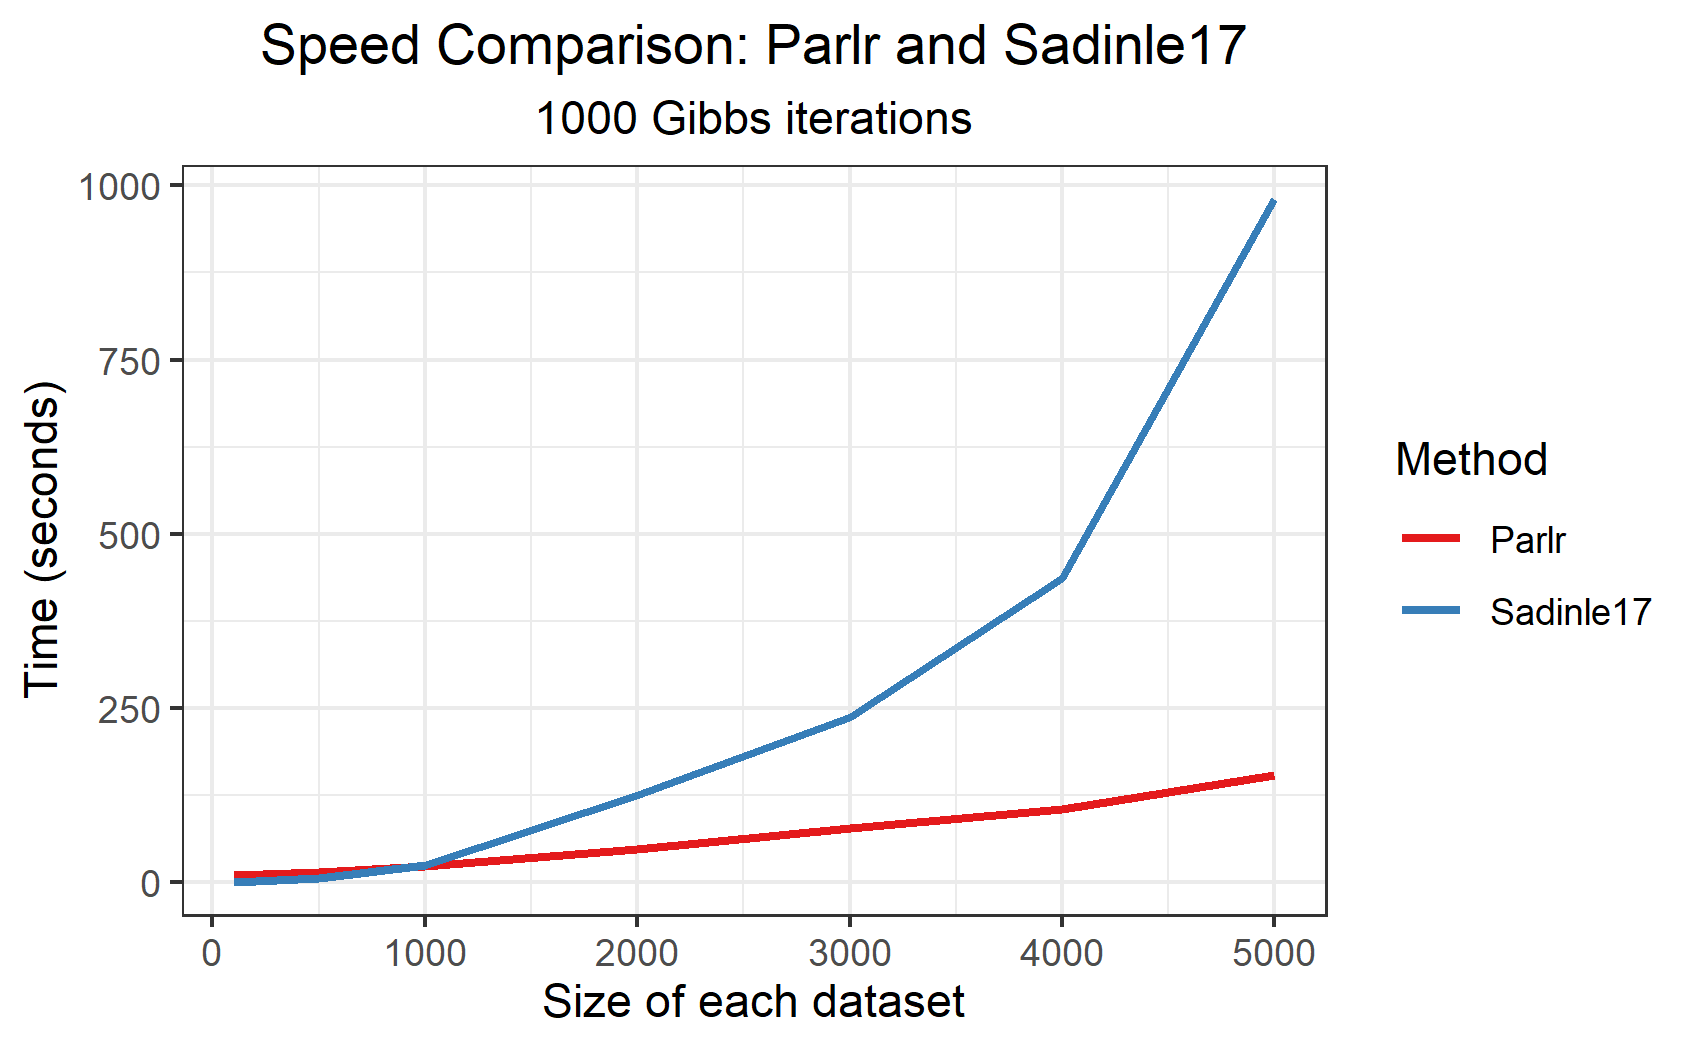
\includegraphics[width=23.6in]{../notes/figures/sadinle_speed_plot} \end{center}

The above discussion suggests that for fixed \(n_B\), computation time
should remain mostly constant with growing \(n_A\). Shockingly, this
seems to be true. In the plot below, fixing \(n_B = 500\), we see linear
growth for the runtime under \texttt{BRL} as \(n_A\) increases, with
much more static runtime under \texttt{parlr}. The slight increases in
runtime that we do see are due primarily to the hashing step, which
again can be run in parallel for large data.

\begin{center}
\includegraphics[width=29.17in]{../notes/figures/speed_plot_fixed_nB} \end{center}

We note here that \texttt{BRL} is coded in C, which makes for unfair
comparison against \texttt{parlr}, currently only built in R.
Additionally, although \texttt{parlr} is amenable to parallezation, this
simulation was run on a single core. Running \texttt{parlr} in C++ with
paralellization for the hashing step and sampling the matching status of
the record pairs should lead to even more drastic results.

\end{document}
